\documentclass{amsart}

% for including graphics
\usepackage{graphicx}

% for tikz picutures
\usepackage[svgnames]{xcolor}
\usepackage{tikz}
\usetikzlibrary{calc}

% for bibliography
\usepackage{biblatex}
\addbibresource{proj2.bib}

% shortcuts
\newcommand{\Ur}{$^{238}$\textrm{U}}
\newcommand{\Ra}{$^{226}$\textrm{Ra}}
\newcommand{\Pb}{$^{210}$\textrm{Pb}}
\newcommand{\Rbar}{\bar{R}}
\newcommand{\Pbar}{\bar{P}}
\newcommand{\Ubar}{\bar{U}}
\newcommand{\Rhobar}{\bar{\rho}}
\begin{document}

\title[Math 481: Project 2]{
  Math 481, Fall 2024\medskip\\
  Project 2\\
  Detecting art forgeries
}

\author{Gabriel Arteaga}
\address{Department of Mathematics and Statistics, UMBC}
\email{garteag@umbc.edu}
\date{October, 12, 2024}

\begin{abstract}
We formulate a system of differential equations corresponding
to evolution in time of a mixture of radioisotopes uranium-238,
radium-226, lead-210, and their eventual conversion to lead-206
which is not radioactive.  We explain how our analysis  may
be applied to detect a forged oil painting.
\end{abstract}

\maketitle

\section{Introduction}
Art forgery has been a prevalent challenge in art for decades, with some forgeries going undetected for years. This means serious financial losses for collectors and museums. A very famous case of this being that of Han van Meegeren~\cite{Braun-DiffEq}, who during his time perfected a method of faking paintings by Johannes Vermeer. His paintings slipped through the cracks until, due to legal pressure, he confessed. However out of all of his paintings, there was one that was still very heavily debated, "Disciples at Emmaus". The reason for this debate being the quality of the painting, van Meegeren's previous work was vastly inferior to this painting and as such must have been authentic. It stayed this way until 1967 when a group of scientists at Carnegie Mellon took the white lead found in paint and used it to date the painting by the quantity of Uranium-238, Radium-226, and Lead-210(Chemical symbols of \Ur, \Ra,\, and \Pb). This is exactly the method that we study in this paper. In Section~\ref{sec:back-info} we look at the background information needed such as half-life and decay rate, as well as deriving a basic solution to a standard decay rate differential equation. In Section~\ref{sec:Half-Life&Decay-Rate} we further discuss half-life and decay rate, as well as calculating decay rates for each isotope. In Section~\ref{sec:math-model} we derive the system of differential equations that describes the decay of \Ra,\, and \Pb,\, over time. Finally in Section~\ref{sec:forgery} we discuss how we will detect a forgery and, using equilibrium states of the three isotopes, verify that our model is consistent with the real world.

\section{Background Information}
\label{sec:back-info}
Before we begin we need some context as to exactly what half-life is. Half-Life is the time it takes for any quantity of any compound to decay to exactly half of its beginning weight. In relation to this is a sample's decay rate, which is the speed at which a sample loses its atoms over time. In this article we define decay rate as $\lambda$ and half-life as $\tau$. Fortunately it is quite simple to find a relation between the two using a standard decay differential equation and we do so below. \\
A standard decay equation gives
\begin{equation} \label{eq:decayequation}
    \frac{dQ(t)}{dt}=-\lambda Q(t),
\end{equation}
    

where $Q(t)$ is the amount of radioactive material for an arbitrary sample. We also define an arbitrary initial value
\[
    Q(0)=Q_{0}.
\]
Solving this initial value problem gives us 
\[
    Q(t)=Q_{0}e^{-\lambda t}.
\]
If we want to solve for the half-life we replace $t$ with $\tau$ , our arbitrary half life, and solve this equation
\[
    \frac{Q_0}{2}=Q_{0}e^{-\lambda \tau}.
\]
We get that
\begin{equation}\label{eq:halflife}
    \tau=\frac{\ln(2)}{\lambda},
\end{equation}
and thus we have our desired relation between half-life and decay rate. With this information we can begin to create our own system.  \\

\section{Half-Life and Decay Rate}
\label{sec:Half-Life&Decay-Rate}
Now we begin with a few definitions, for half-life we define, 
\[
    \tau_U, \text{  } \tau_R, \text{   } \tau_P,
\]
and for decay rate
\[
    \lambda_U, \text{  } \lambda_R, \text{   } \lambda_P,
\]
for \Ur,\, \Ra,\,\Pb, \,respectively.\\\\

We now aim to calculate the decay rates using data from~\cite{wiki-U238,wiki-ra226,wiki-pb210}. This gives us the following half-life for each substance,
\begin{align*}
    &\tau_U=	4.5\times10^9 \text{ years},\\
    &\tau_R= 1600 \text{ years},\\
    &\tau_P= 22 \text{ years}.
\end{align*}
Recalling equation~\eqref{eq:halflife} we can re-arrange for $\lambda$,
\[
    \lambda=\frac{\ln(2)}{\tau}.
\]
Plugging in values for half-life we arrive at the decay rates,
\begin{align*}
    &\lambda_U=	1.54\times10^{-10} \text{ years}^{-1},\\
    &\lambda_R= 4.33\times10^{-4} \text{ years}^{-1}, \\
    &\lambda_P= 0.031 \text{ years}^{-1} . 
\end{align*}


\section{Mathematical Model}\label{sec:math-model}
Now we may begin making the model itself. First we notice the half-life of \Ur\, that being roughly $4.5$ billion years far beyond the scope of this paper. Due to this we will assign \Ur\, to be a constant value, that of $U$. Recalling our decay equation~\eqref{eq:decayequation} we can come to,
\[
    \frac{dR(t)}{dt}=-\lambda_R R(t). 
\]
However we must account for the fact that more \Ra\, is being produced by \Ur\, decaying. So we add a term to account for this increase,
\begin{equation}\label{eq:radiumdiff}
    \frac{dR(t)}{dt}=-\lambda_R R(t)+\lambda_U U.
\end{equation}
We do the same for \Pb\, accounting for \Ra\, decaying instead of \Ur\,,
\begin{equation}\label{eq:leaddiff}
    \frac{dP(t)}{dt}=-\lambda_P P(t)+\lambda_R R(t).
\end{equation}
This will be our system of differential equations for the rest of the paper. 
\section{Detecting a forgery}\label{sec:forgery}

To detect if a painting is a forgery or not we must first understand how the paint was attained. At some point this lead ore was all \Ur,\, and over time it decays becoming, \Ra,\, then finally we arrive at \Pb.\, This is also the reason that we only shift our attention to the three specific isotopes. At the stage it is ore all three isotopes are at equilibrium, we say in this state the quantities are at, $\Ubar\,$$, \Rbar\,$, and $\Pbar\,$. It is then mined and smelted in order to extract the lead that is used as a pigment for white paint. At that point only a small quantity of $\Ubar\,$, and $\Rbar\,$, is left we call this factor $\alpha$.  We provide a diagram that helps with understanding these states below. 

\begin{figure}
    \centering
    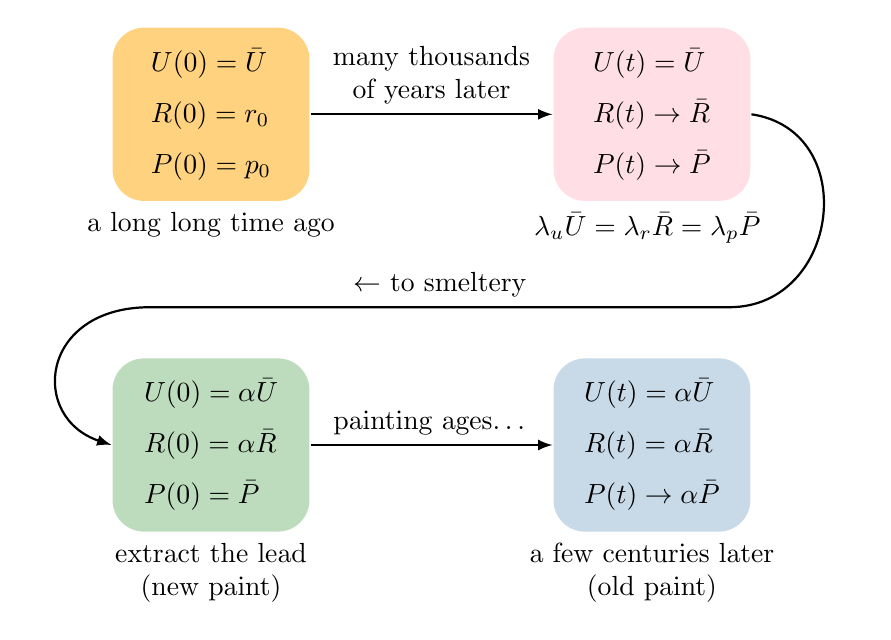
\begin{tikzpicture}[>=latex, scale=0.7, thick]
    
        \begin{scope}
            \node[fill=Orange!50,
                rounded corners=4mm, minimum width=25mm, minimum height=22mm]
                (Box1) at (9,0) {};
            \node[align=left] at (Box1)
                { $U(0)=\bar{U}$ \\[1.5ex] $R(0)=r_0$ \\[1.5ex] $P(0)=p_0$ };
            \node[below, align=center] at (Box1.south)
                {a long long time ago};
        \end{scope}

        \begin{scope}[xshift=8cm]
            \node[fill=Pink!50,
                rounded corners=4mm, minimum width=25mm, minimum height=22mm]
                (Box2) at (9,0) {};
            \node[align=left] at (Box2)
                { $U(t) = \bar{U}$ \\[1.5ex] $R(t) \to \bar{R}$ \\[1.5ex]
                    $P(t) \to \bar{P}$ };
            \node[below, align=center] at (Box2.south)
                {$\lambda_u \bar{U} = \lambda_r \bar{R} = \lambda_p \bar{P}$ };
        \end{scope}

        \begin{scope}[yshift=-6cm]
            \node[fill=ForestGreen!30,
                rounded corners=4mm, minimum width=25mm, minimum height=22mm]
                (Box3) at (9,0) {};
            \node[align=left] at (Box3)
                { $U(0)=\alpha \bar{U}$ \\[1.5ex]
                    $R(0)=\alpha \bar{R}$ \\[1.5ex]
                    $P(0)=\bar{P}$ };
            \node[below, align=center] at (Box3.south)
                {extract the lead\\(new paint)};
        \end{scope}

        \begin{scope}[xshift=8cm, yshift=-6cm]
            \node[fill=SteelBlue!30,
                rounded corners=4mm, minimum width=25mm, minimum height=22mm]
                (Box4) at (9,0) {};
            \node[align=left] at (Box4)
                { $U(t)=\alpha \bar{U}$ \\[1.5ex]
                    $R(t)=\alpha \bar{R}$ \\[1.5ex]
                    $P(t) \to \alpha\bar{P}$ };
            \node[below, align=center] at (Box4.south)
                {a few centuries later\\(old paint)};
        \end{scope}

        \draw[->] (Box1.east)
            -- node[above, align=center] {many thousands\\of years later}
            (Box2.west);

        \draw[->] (Box2.east)
            .. controls +(2.0,-0.3) and +(2.0,0) .. +(-0.4,-3.5)
            .. controls +(-2.0,0) and +(2.0,0) ..
            node[above] {$\leftarrow$ to smeltery} ($(Box3.west) +(0.7,2.5)$)
            .. controls +(-2,0) and +(-1.5,0.5)
            .. (Box3.west);

        \draw[->] (Box3.east)
            -- node[above] {painting ages\ldots}
            (Box4.west);

    \end{tikzpicture}
    \caption{Visual description of the change the uranium-238, radium-226, and lead-210 experience over time .}
    \label{fig:decay-schematics}
\end{figure}










To begin our calculations we assume that the ore begins at an equilibrium state. That means that our initial conditions for our system of differential equations is given by the equilibrium state equation for \Ra,\, and \Pb.\, If the system is indeed in equilibrium then,
\begin{align*}
    &\frac{dR}{dt}=0\\
    &\frac{dP}{dt}=0.
\end{align*}
We denote our equilibrium states with $\Ubar$, $\Rbar$, and $\Pbar$. Using our definitions of~\eqref{eq:radiumdiff}~\eqref{eq:leaddiff}, we get the equations, 
\begin{align*}
    &-\lambda_R\Rbar+\lambda_U \Ubar=0\\
    &-\lambda_P \Pbar+\lambda_R \Rbar=0.
\end{align*}
Further simplification gives us,
\begin{align*}
     &\lambda_R\Rbar=\lambda_U \Ubar=\lambda_P \Pbar.\\
\end{align*}
Furthermore this gives us our desired $\Rbar$, and $\Pbar$ at equilibrium
\begin{equation}\label{eq:Req}
\begin{aligned}
    &\Rbar=\frac{\lambda_U \Ubar}{\lambda_R}\\
    &\Pbar=\frac{\lambda_U \Ubar}{\lambda_P}.
\end{aligned}
\end{equation}
We now define some differential equations to see how these quantities change over time. These will be much like equations~\eqref{eq:radiumdiff} and~\eqref{eq:leaddiff} however we must now consider for the smaller amount of \Ra\,  and \Ur.\, We come to 
\begin{equation} \label{eq:alRaDiff}
\left\{
\begin{aligned}
    &\frac{dR(t)}{dt}=-\lambda_RR(t)+\alpha\lambda_UU\\
    &\frac{dP(t)}{dt}=-\lambda_PP(t)+\lambda_RR(t).
\end{aligned}
\right.
\end{equation}
Note two things, first in this system uranium is still constant. As noted in Section~\ref{sec:Half-Life&Decay-Rate} the half-life of uranium will practically stay constant throughout the segment of time that we are interested in. Secondly note that there is no inclusion of $\alpha$ in the differential equation for \Pb,\, in the process of smelting we recover the full quanity of \Pb, therefore it should not change from it's quantity in the state of ore. With this in mind we define the initial conditions for this system. As our system begins in equilibrium then we take $\Rbar$ and $\Pbar$ as our initial conditions, with that our system becomes
\begin{equation}\label{eq:diffsys}
\left\{
\begin{aligned}
&\frac{dR(t)}{dt}=-\lambda_RR(t)+\alpha\lambda_UU, \, R(0)=\alpha\Rbar \\ 
&\frac{dP(t)}{dt}=-\lambda_PP(t)+\lambda_RR(t),\, P(0)=\Pbar.
\end{aligned}
\right.
\end{equation}
Using Maple we solve our system to get, 

\begin{equation}
\left\{
\begin{aligned}
    &R(t)=\frac{\alpha \lambda_U U}{\lambda_P}\\
    &P(t)=\frac{-e^{(-\lambda_Pt)} \lambda_U U(\alpha-1)+\alpha\lambda_UU)}{\lambda_P}.
\end{aligned}
\right.
\end{equation}
We will now analyse the ratio of these two, which if the painting is real will look exactly the same as the ratio in equilibrium. If not then the ratio in the system will diverge from what the equilibrium gives us. We define these ratios as 
\begin{equation}\label{eq:rhofunct}
        \rho(t)=\frac{P(t)}{R(t)}=-\frac{(\alpha-1)\lambda_R(e^{(-\lambda_Pt)})}{\lambda_P\alpha}+\frac{\lambda_R}{\lambda_P}
\end{equation}
and, 
\begin{equation}
    \Rhobar=\frac{\Pbar}{\Rbar}=\frac{\lambda_R}{\lambda_P}.
\end{equation}
We now recall our expression for each $\lambda$, along with each respective half-life or $\tau$, in Section~\ref{sec:Half-Life&Decay-Rate}, namely
\begin{align*}
     &\lambda_R=\frac{\ln(2)}{1600},\\
     &\lambda_P=\frac{\ln(2)}{22}.
\end{align*}
This gives us that,
\[
\Rhobar=\frac{11}{800}.
\]
So we want to confirm that the limit as $t$ goes to infinity correlates with this number. To do this we first must give $\alpha$ some numerical quantity, we give it the value of $10^{-4}$. We then calculate this limit to get, 
\begin{equation}
\lim_{t\to\infty}\rho(t)=\frac{11}{800}.
\end{equation}
This is the exact quantity of $\Rhobar$, represented visually below. With this we are assured that our model is consistent with a standard equilibrium.

\begin{figure}
    \centering
    \includegraphics[width=0.8\linewidth]{rhograph.png}
    \caption{$\rho$ is marked in blue, while $\Rhobar$ is in red representing what we want $\rho$ to converge to.}
    \label{fig:enter-label}
\end{figure}

\section{Conclusion}
In this paper we have detailed the mathematical process in which art forgery is detected. More specifically the method in which Han van Meegeren's "Disciples at Emmaus" was detected. We did this by analysing the ratio of \Pb,\, and \Ra.\, We found these quantities through a system of differential equations that modeled the decay of the two isotopes over time. Finally confirming that our model was accurate by obtaining our same ratio but in terms of the equilibrium states and seeing that it matched with real world expectations. With this model we may check other paintings in the future, given that they use lead based paints, to strengthen the integrity of art. 
\printbibliography

\end{document}

